\documentclass[12pt,fleqn,answers]{exam}
\usepackage{pifont}
\usepackage{dingbat}
\usepackage{amsmath,amssymb}
\usepackage{epsfig}
\usepackage{upgreek}
\usepackage[super]{nth}
\usepackage[colorlinks=true,linkcolor=black,anchorcolor=black,citecolor=black,filecolor=black,menucolor=black,runcolor=black,urlcolor=black]{hyperref}
\usepackage[letterpaper, margin=0.75in]{geometry}
\addpoints
\boxedpoints
\pointsinmargin
\pointname{pts}

\usepackage[activate={true,nocompatibility},final,tracking=true,kerning=true,factor=1100,stretch=10,shrink=10]{microtype}
\usepackage[american]{babel}
%\usepackage[T1]{fontenc}
\usepackage{fourier}
\usepackage{isomath}
\usepackage{upgreek,amsmath}
\usepackage{amssymb}
\usepackage{graphicx}

\newcommand{\dotprod}{\, {\scriptzcriptztyle
    \stackrel{\bullet}{{}}}\,}

\newcommand{\reals}{\mathbf{R}}
\newcommand{\lub}{\mathrm{lub}} 
\newcommand{\glb}{\mathrm{glb}} 
\newcommand{\complex}{\mathbf{C}}
\newcommand{\dom}{\mbox{dom}}
\newcommand{\range}{\mbox{range}}
\newcommand{\cover}{{\mathcal C}}
\newcommand{\integers}{\mathbf{Z}}
\newcommand{\vi}{\, \mathbf{i}}
\newcommand{\vj}{\, \mathbf{j}}
\newcommand{\vk}{\, \mathbf{k}}
\newcommand{\bi}{\, \mathbf{i}}
\newcommand{\bj}{\, \mathbf{j}}
\newcommand{\bk}{\, \mathbf{k}}
\DeclareMathOperator{\Arg}{\mathrm{Arg}}
\DeclareMathOperator{\Ln}{\mathrm{Ln}}
\newcommand{\imag}{\, \mathrm{i}}

\usepackage{graphicx}
\usepackage{color}
\shadedsolutions
\definecolor{SolutionColor}{rgb}{0.8,0.9,1}
\newcommand\AM{\textsc{am}}
\newcommand\PM{\textsc{pm}}
     
\newcommand{\quiz}{3}
\newcommand{\term}{Fall}
\newcommand{\due}{Wednesday 7 September 13:15 \PM}
\newcommand{\class}{MATH 115}
\begin{document}
\large
\vspace{0.1in}
\noindent\makebox[3.0truein][l]{\textbf{\class}}
\textbf{Name:} \hrulefill \\
\noindent \makebox[3.0truein][l]{\textbf{In class work \quiz, \term \/ \the\year}}
\textbf{Row and Seat}:\hrulefill\\
\vspace{0.1in}


\noindent  In class work  \quiz\/  has questions 1 through  \numquestions \/ with a total of  \numpoints\/  points.   
Turn in your work at the end of class  \emph{on paper}. This assignment is due \emph{\due}.

\vspace{0.1in}


\begin{questions} 

\question Find each of the following limits. Justify each of your 
steps by referencing one of our rules numbered zero through seven.

\begin{parts}
  
    \part[2] \(\displaystyle \lim_{x \to \uppi} \left(x^3 + x \right) \)
    \begin{solution}[1.5in]
        Since $x^3 + x$ is a polynomial, we can use Rule 6; thus
        \begin{align*}
            \lim_{x \to \uppi} \left(x^3 + x \right) &= \uppi^3+\uppi. \hfill &\mbox{(Rule 6)}
        \end{align*}
        Alternatively, we could first use Rule 1 (linearity) followed by
        Rule 4; thus
        \begin{align*}
            \lim_{x \to \uppi} \left(x^3 + x \right) &=   \lim_{x \to \uppi} (x^3) +  \lim_{x \to \uppi} (x), \hfill &\mbox{(Rule 1)}\\
                      &= \uppi^3+\uppi. \hfill  &\mbox{(Rule 4, twice)}
        \end{align*}
        To apply Rule 4 to \(\displaystyle \lim_{x \to \uppi} (x)\), match to the 
        algebraically equivalent \(\displaystyle \lim_{x \to \uppi} (x^1)\).
    \end{solution}
      
    \part[2] \(\displaystyle  \lim_{x \to \sqrt{2}} \sqrt{x+1} \)
    \begin{solution}[1.5in]
        We have
        \begin{align*}
            \lim_{x \to \sqrt{2}} \sqrt{x+1} &= \sqrt{\lim_{x \to \sqrt{2}} (x+1)}, &\mbox{(Rule 5)} \\
                                             &= \sqrt{1 + \sqrt{2}}. &\mbox{(Rule 6)}
        \end{align*}
        Since $x+1$ is a polynomial, using Rule 6 in the second step is OK.
    \end{solution}

    \part[2] \(\displaystyle  \lim_{x \to \sqrt{2}} \frac{x+1}{x-1} \)
    \begin{solution}[1.5in]
        We have
        \begin{align*}
            \lim_{x \to \sqrt{2}} \frac{x+1}{x-1} &= \frac{\sqrt{2}+1}{\sqrt{2}-1},  &\mbox{(Rule 7)} \\
                                                  &= 3 + 2 \sqrt{2}. &\mbox{(simplification)}
        \end{align*}
        The simplification step is done using a multiply by one trick:
        \begin{align*}
            \frac{\sqrt{2}+1}{\sqrt{2}-1} &= \frac{\sqrt{2}+1}{\sqrt{2}-1} \times \frac{\sqrt{2}+1}{\sqrt{2}+1}, 
            \hfill &\mbox{(multiply by one)}\\
                &= \frac{(\sqrt{2}+1)^2}{2 + \sqrt{2} - \sqrt{2} - 1}, \hfill &\mbox{(distribute denominator)}\\
                &= \frac{(\sqrt{2}+1)^2}{1}, \hfill &\mbox{(collect like terms)}\\
                &= 2 + 2\sqrt{2}+1, \hfill &\mbox{(divisor of one)}\\
                &= 3 + 2 \sqrt{2}. \hfill &\mbox{(collect like terms)}
        \end{align*}
        To earn full credit with our online homework system, generally
        removing radicals from denominator is required.

    \end{solution}

    \part[2] \(\displaystyle  \lim_{x \to 35} \sqrt{12 -2 \sqrt{x}} \)
    \begin{solution}[1.5in]
        We have
        \begin{align*}
            \lim_{x \to 35} \sqrt{12 -2 \sqrt{x}} &= \sqrt{\lim_{x \to 35} (12 -2 \sqrt{x}) } , &\mbox{(Rule 5)} \\
               &= \sqrt{\lim_{x \to 35} (12)  -2 \lim_{x \to 35} \sqrt{x} } , &\mbox{(Rule 1)} \\
               &= \sqrt{12  -2 \sqrt{35}} , &\mbox{(Rule 0, Rule 5)} \\
               &= \sqrt{7}-\sqrt{5}. &\mbox{(simplification)}
        \end{align*}
        The simplification in the last step is an application of the square
        root denesting identity
        \[
            \left(\forall a,b \in \reals_{\geq 0} \right) 
              \left(\sqrt{a+b-2\sqrt{ab}} = \sqrt{\max(a,b)} - \sqrt{\min(a,b)} \right).
        \]
        And no, such simplifications are \emph{not} required (but it is cute).
        
        
        \quad You'll be happy to know that denesting radicals is one of my hobbies. Some time ago, as a challenge
        from a friend, I denested
        \[
            2028 \times (2 \times 3^{5/2} \, \mathrm{i} +35)^{1/3}-(2 \times 3^{5/2} \, \mathrm{i}+35)^{2/3} \times (8 \times 3^{7/2} \mathrm{i}-420)+10140.
        \]
        to the integer 24336. To do this, in part, I used an algorithm 
        that was invented by the mathematician turned artist Helaman Ferguson \url{https://en.wikipedia.org/wiki/Helaman_Ferguson}
    \end{solution}


\end{parts}

%\newpage

\question A graph of a function $Q$ is shown. Using the graph,
as best you can find the numerical value of each limit.

\begin{parts}
    \part [1] \(\displaystyle \lim_{x \to 2} Q(x) \)
    \begin{solution}[1.5in]
        Looking at the graph, it appears that when the input
        is close to 2, the output is close to 2. Moving closer
        to two from either the left or the right, the output grows
        ever closer to two. Thus, visual evidence suggests that
        \[
            \lim_{x \to 2} Q(x) = 2.
        \]
        The visual evidence \textbf{isn't} a proof. Maybe if we zoomed in on
        the graph magnifying by a factor of trillions, that maybe 
        the graph will wiggle around in some crazy way near the 
        limit point. 
        
    \end{solution}
    \part [1] \(\displaystyle \lim_{x \to -1^{(+)}} Q(x) \)
    \begin{solution}[1.5in]
        Remember that the special notation $-1^{(+)}$ means that
        the limit point is $-1$, but we only consider inputs that
        are \emph{larger} (or to the right) of $-1$. Immediately
        to the right of the limit point, the output of the
        $Q$ appears to be a constant $2$. Thus, the visual evidence
        is that \(\displaystyle \lim_{x \to -1^{(+)}} Q(x) = 2\).

        Once again, visual evidence \textbf{isn't} a proof.

        
    \end{solution}

\end{parts}

\begin{center}
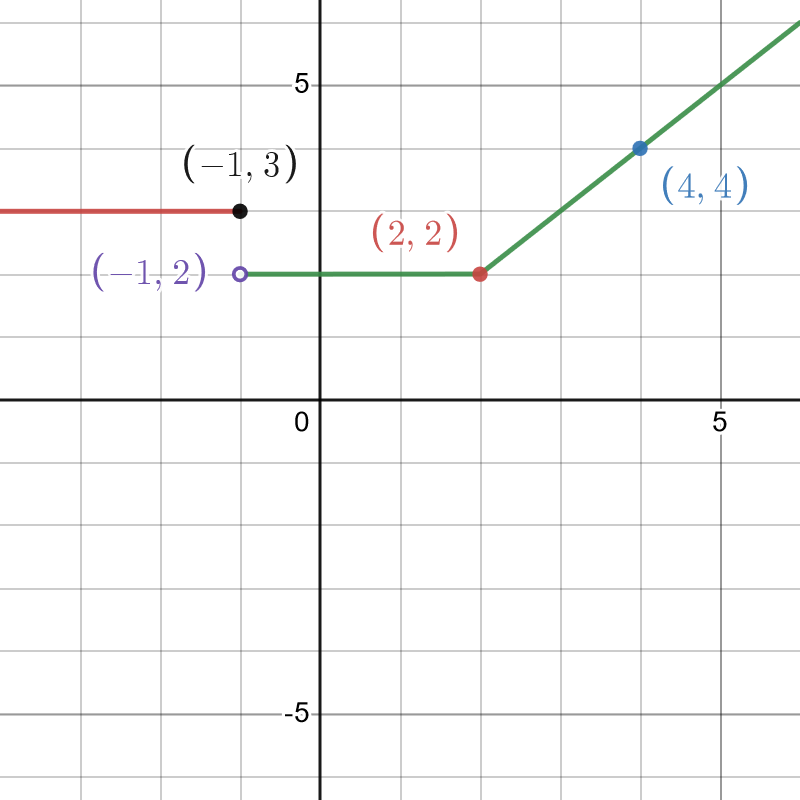
\includegraphics[scale=0.25]{desmos-graph(28).png}
\end{center}

\end{questions}

\newpage
\noindent Suppose functions $F$ and $G$ have limits toward $c$ and suppose $a,b \in \reals$ and $n$ is a positive integer. Then

\begin{description}

\item[Rule \#0 (constant)] $  \displaystyle \lim_{x \to c} (a) = a$.
 
\item[Rule \#1 (linearity)] $ \displaystyle \lim_{x \to c} (a F(x) + b G(x)) = a  \, \lim_{x \to c} (F(x)) + b \, \lim_{x \to c} (G(x)) $.

\item [Rule \#2 (product)]$ \displaystyle \lim_{x \to c} (F(x)  G(x)) = \, \lim_{x \to c} (F(x))  \times \lim_{x \to c} (G(x)) $.

\item [Rule \#3 (quotient)] Provided $\displaystyle  \lim_{x \to c} (G(x)) \neq 0$, we have $\displaystyle \lim_{x \to c} \frac{F(x)}{G(x)} = \, \frac{\lim_{x \to c} (F(x))}{ \lim_{x \to c} (G(x)) } $.

\item [Rule \#4 (power)]  $ \displaystyle \lim_{x \to c} F(x)^n  = \left(\lim_{x \to c} F(x) \right)^n  $.

\item [Rule \#5 (root)]  Provided $ \displaystyle  \left(\lim_{x \to c} F(x) \right)^{1/n} $ is real,  $ \displaystyle \lim_{x \to c} F(x)^{1/n}  = \left(\lim_{x \to c} F(x) \right)^{1/n}  $.

\item [Rule \#6 (polynomial)]  Provided $F$ is a polynomial, we have  $ \displaystyle \lim_{x \to c} F(x) = F(c)$

 \item [Rule \#7 (rational)]  Provided $F$ is a rational function and $c \in \dom(F)$, we have  \mbox{$ \displaystyle \lim_{x \to c} F(x) = F(c)$.}
\end{description}
\end{document}